\paragraph{biguint-add}

\subparagraph{Target}
Implement the addition of two biguints.

\subparagraph{Constraints logic}
\begin{itemize}
    \item Equation for gates;
    \item Sumcheck between output and limbs;
    \item Rangecheck for limbs.
\end{itemize}

\subparagraph{Circuit layout}
See \figref{fig:biguint-add-circuit-layout}.
\begin{figure}[!ht]
    \centering
    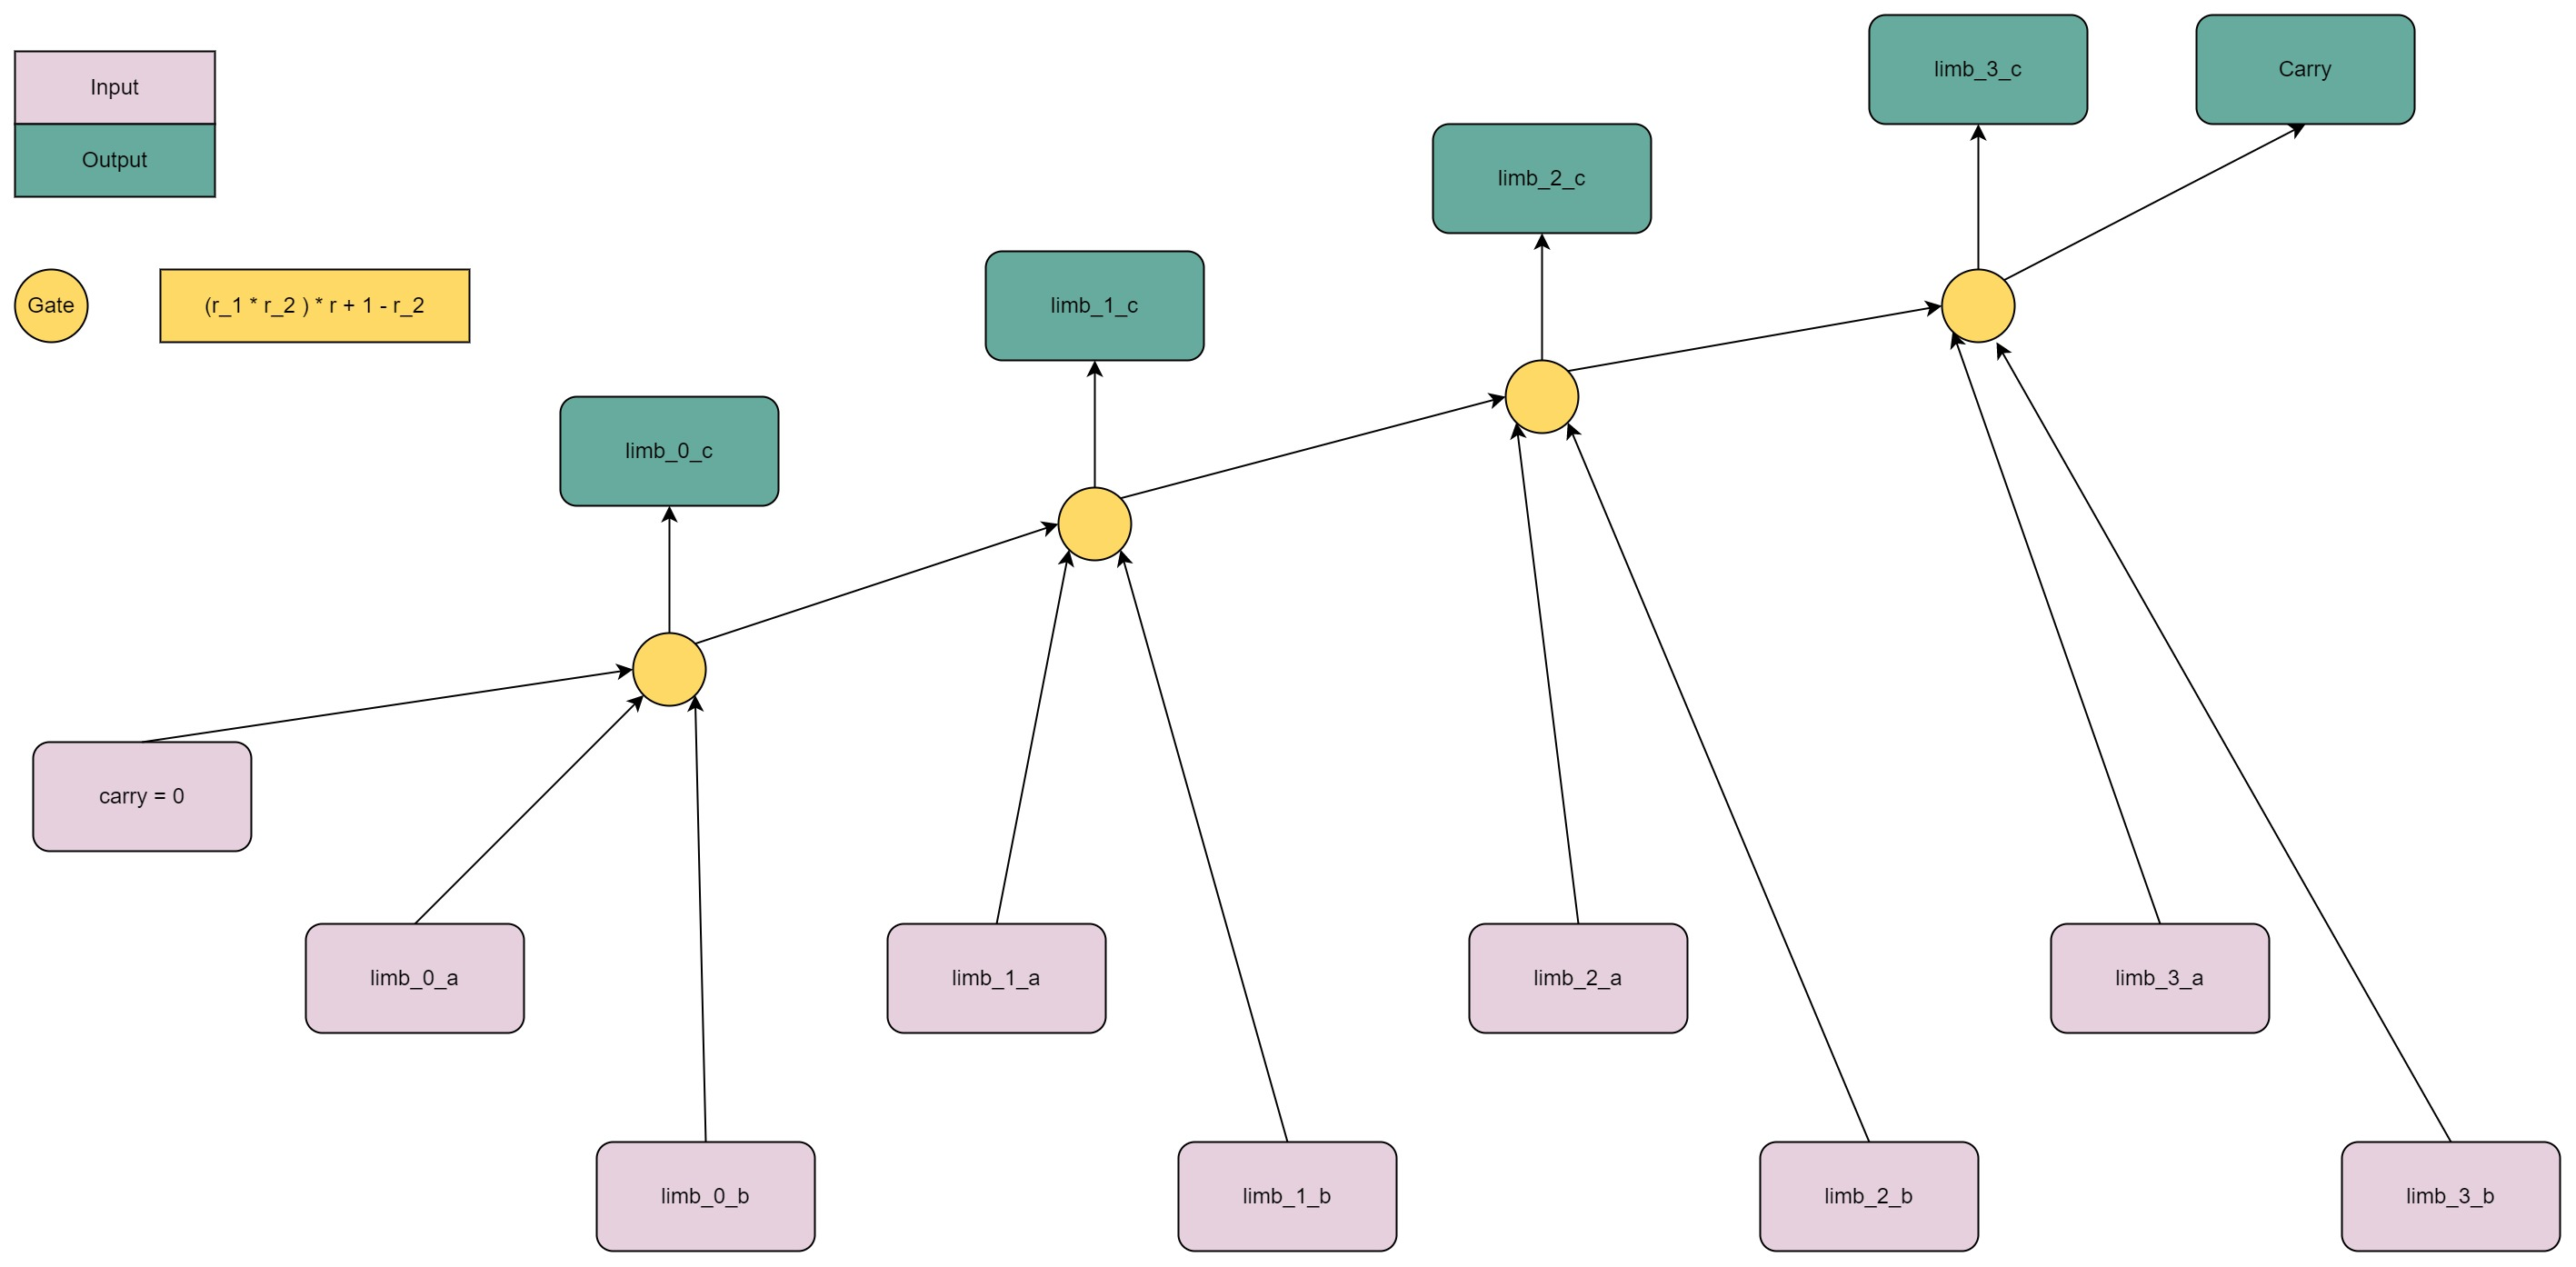
\includegraphics[width=0.5\textwidth]{biguint-add-circuit-layout.jpg}
    \caption{biguint-add circuit layout}
    \label{fig:biguint-add-circuit-layout}
\end{figure}

\subparagraph{Trace layout}
See \figref{fig:biguint-add-trace-layout}.
\begin{figure}[!ht]
    \centering
    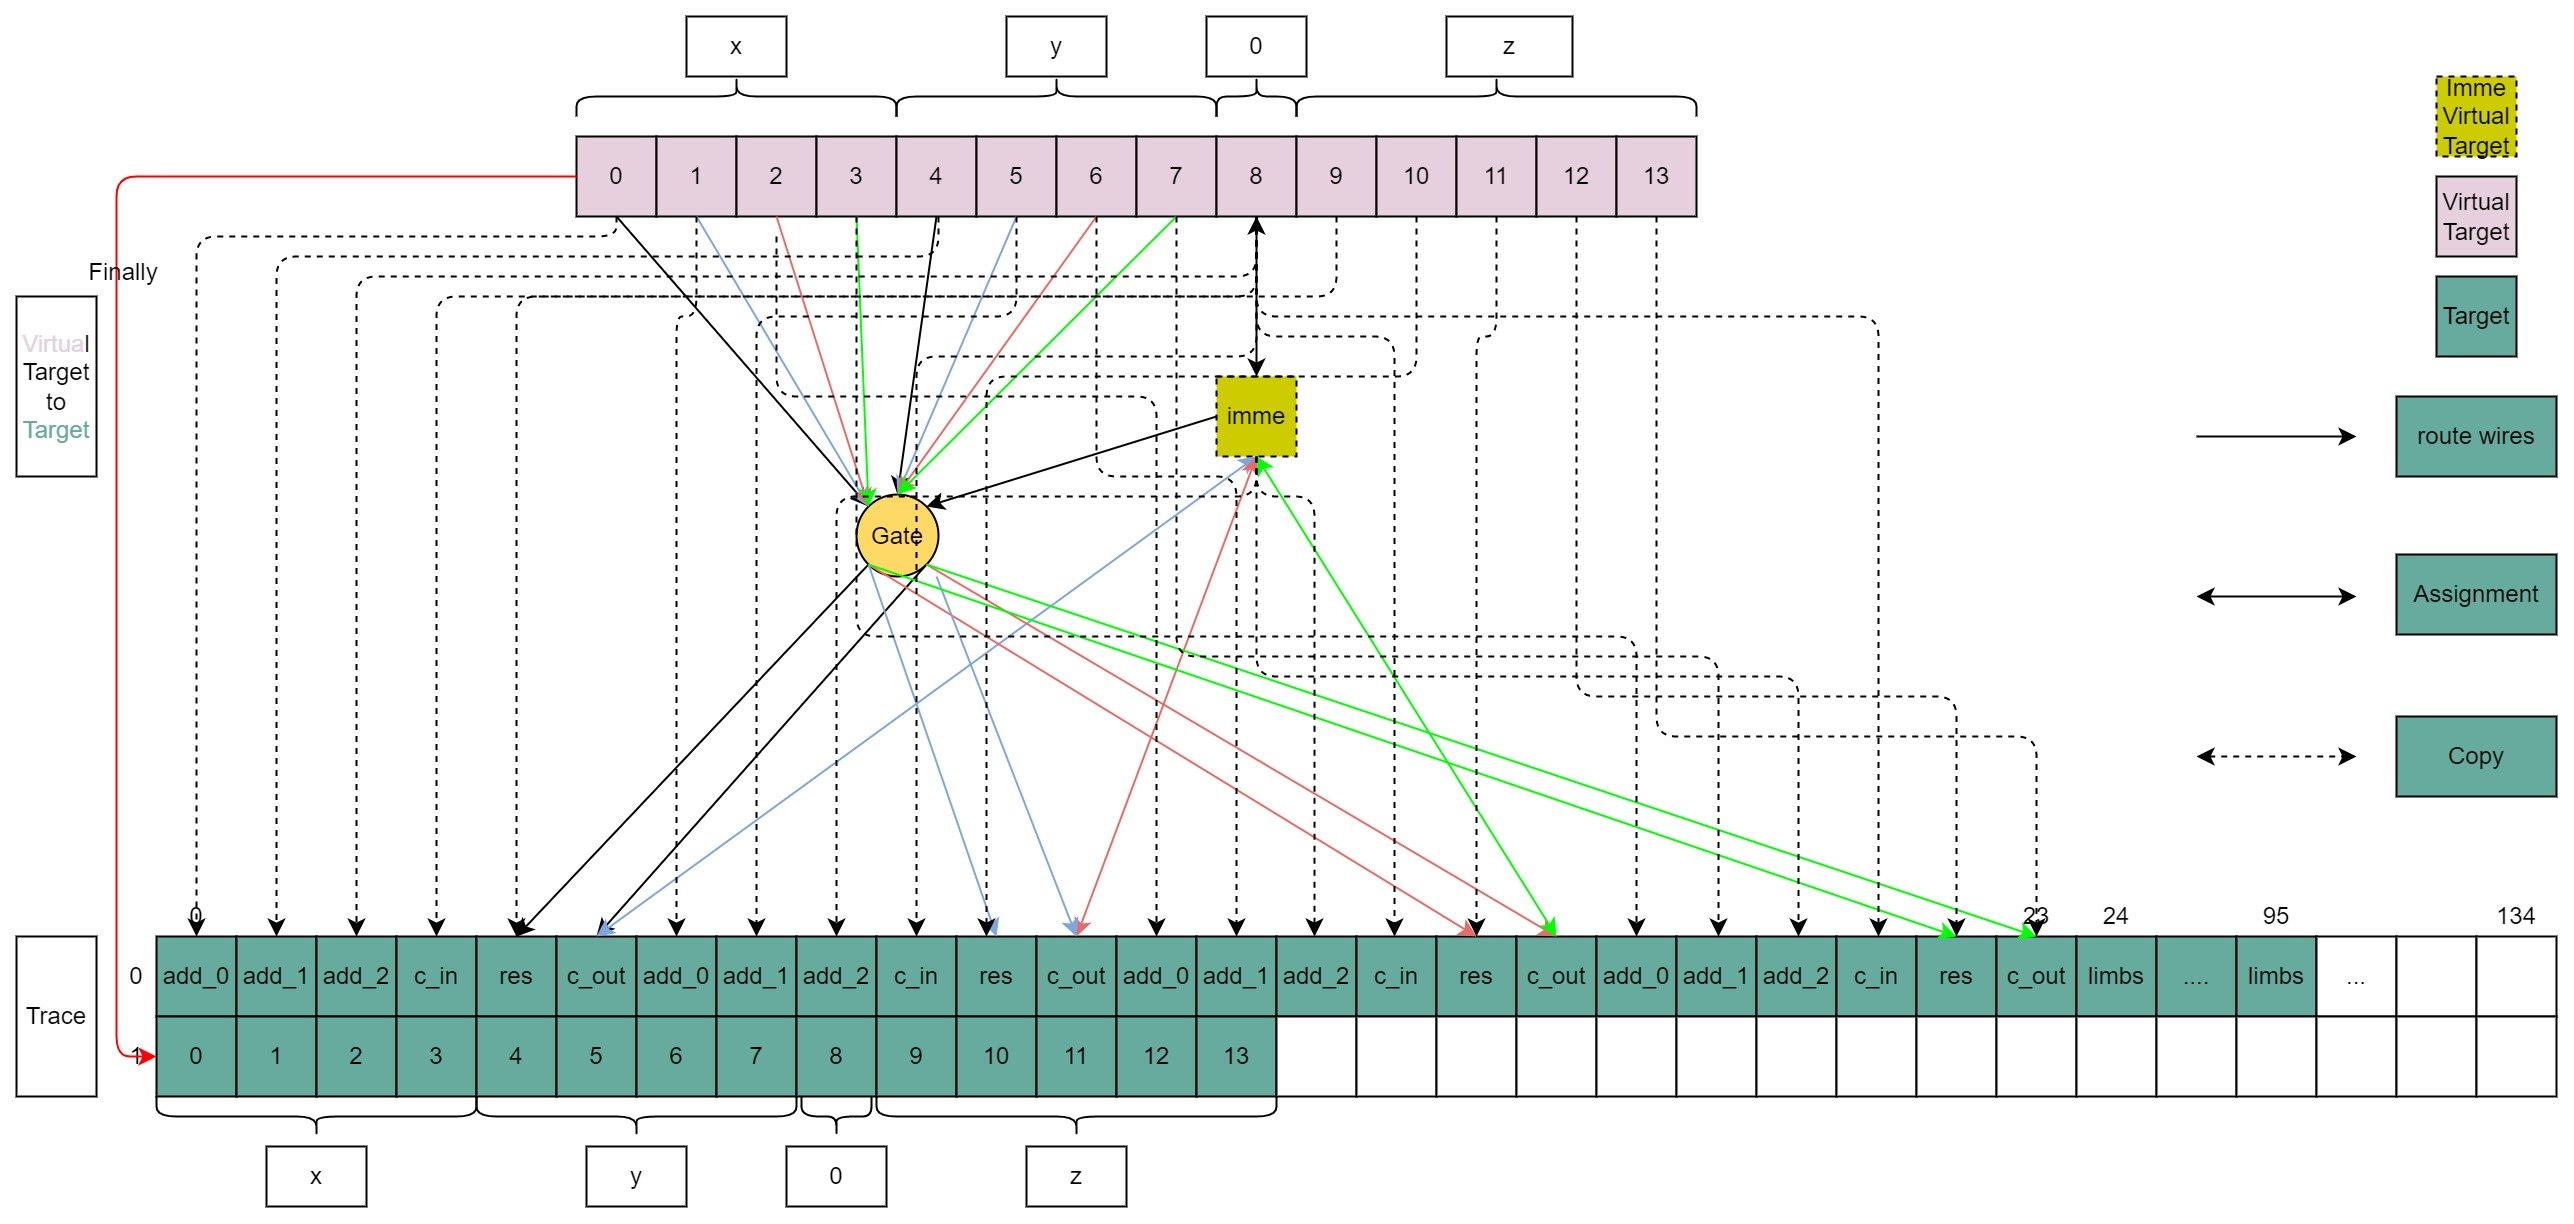
\includegraphics[width=0.5\textwidth]{biguint-add-trace-layout.jpg}
    \caption{biguint-add trace layout}
    \label{fig:biguint-add-trace-layout}
\end{figure}

\subparagraph{Constraints info and costs}
\begin{itemize}
    \item gate type num: 1 (U32AddManyGate)
    \item gate ops num: limbs-num
    \item gate instance num: ceil(limbs-num / gate.ops)
    \item copy-constraints: limbs-num * 4
    \item max-degree: 4 (\verb|1 << limb-bits|)
\end{itemize}

\subparagraph{Questions}
\begin{itemize}
    \item Why not make rangecheck constraint for inputs?
    \item Why not make copy constraint between cur-c-in and last-c-out?
\end{itemize}
